\documentclass[11pt, oneside]{book}
\newcommand{\version}{v2}

\begin{document}
\usepackage[pdftex,a4paper]{geometry}
\usepackage{pdfpages}
\usepackage{graphicx}
\usepackage{amssymb}
\usepackage{gensymb}
\usepackage{eurosym}
\usepackage{ifthen}
\usepackage{float}
\usepackage{calc}
\usepackage[export]{adjustbox}% http://ctan.org/pkg/adjustbox
\usepackage{xstring}
\usepackage{multicol}
\usepackage[framemethod=TikZ]{mdframed}
\usepackage[T1]{fontenc}

% Switch font comprehensively
\usepackage[scaled]{helvet}
\renewcommand\familydefault{\sfdefault} 

% Use as much of the page as we can.
\pagestyle{empty}
\setlength{\parindent}{4em}
\setlength{\parskip}{1.2em}
\setlength{\textheight}{28cm}
\setlength{\textwidth}{19cm}
\setlength{\hoffset}{-2cm}
\setlength{\voffset}{-2cm}

% DECAL function
%
% The decal function takes 5 inputs and extracts a symbol from the Italian ISO document that is included in this repository. The function then displays the symbol together with the title and warning text.
%
% Parameters:		#1 Page with the symbol on it in the document.
%			#2 Title
%			#3 Y height on the page.
%			#4 X location on the page. (not sure on this)
%			#5 Warning subtext
%
\newcommand{\decal}[5]{
\begin{minipage}{\linewidth}
	\begin{minipage}[t]{0.3\textwidth}
	       \vspace{0pt}
	       % The ISO document has a 'gutter' - so we shift the X a bit on the left/right page.
	       %
		\ifthenelse{\isodd{#1}}{ %if the pagenumber is odd, use this location for the image
			\includegraphics[width=0.9\textwidth,page=#1,viewport=103 #3 291 #4,clip=true]{./media/13GR_PistopioimeniSimansi_ISO_7010.pdf}
		}{ %else (because the pagenumber is even), use this location for the image.
			\includegraphics[width=0.9\textwidth,page=#1,viewport=70 #3 261 #4,clip=true]{./media/13GR_PistopioimeniSimansi_ISO_7010.pdf}
		}
	\end{minipage}
	\begin{minipage}[t]{0.6\textwidth}
		\setlength{\parindent}{4em}
		\setlength{\parskip}{1.2em}
	       \vspace{0pt}\raggedright
		{\LARGE \textbf{#2}} %include title text in bold and such
	
		#5 %include warning subtext
		\vspace{0.5cm}
	\end{minipage}
\end{minipage}
}


% Some home made symbols which are not part of the official ISO list of symbols:
%
% Two person symbol
\newcommand{\twopersons}{
\raisebox{-.5\height}{
\includegraphics[width=6mm]{./media/FileAiga_toiletsq_men}}\textbf{x 2} 
}

% Some home made symbols which are not part of the official ISO list of symbols:
% Clock with 7-19 symbol
%
\newcommand{\seventoseven}{
\raisebox{-.5\height}{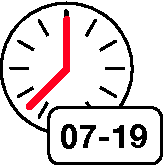
\includegraphics[width=10mm]{./media/clock-limits}}
}


% Define classes for Action, Prohibit and Warn. These each take three inputs.
%
% Turns out that the symbols extracted from the ISO document with \decal are a bit 
% shifted in the Y position or size depending on what class they are. So we split
% them into the three sections that have height differences.
%
% Parameters:		Page with the symbol on it. Actual pagenumber, not the number on the page!
%			Title
%			Warning subtext
%
\newcommand{\action}[3]{\decal{#1}{#2}{520}{715}{#3}}
\newcommand{\prohib}[3]{\decal{#1}{#2}{495}{690}{#3}}
\newcommand{\warn}[3]{\decal{#1}{#2}{520}{715}{#3}}

%% Command to create a round box to call extra attention to something.
%%
\newcommand{\smallicontext}[2]{%
\begin{mdframed}[roundcorner=4pt] 
\begin{tabular}{lp{0.8\linewidth}}
#1 & #2 \\
\end{tabular}
\end{mdframed}
}

% machinePage
% A full page with a machine on it. Takes 5 inputs.
%
% Params:		#1 Machine name
%			#2 Tokens for standard instrutions: Zero or more from
%				Approval	Trustee approval needed.
%				Noise		Not after 19:00
%				Two		Two people required
%				Log		use must be logged
%				Dewalt		Attach dewalt dutch extractor.
%			#3 Specific instructions - added to the above text.
%			#4 Warnings, Symbols - main symbols on page.
%			#5 Extra footer/bottom of the page text
%
\newcommand{\machinePage}[5]{%
\begin{center}
	\vspace{0cm}
	{\fontsize{50}{60} \textbf{#1}}%Machine name
 
	\action{49}{% Determines if you require Induction / the tool has mandatory instructions / or general safety instructions
		\textbf{%
 			\IfSubStr{#2}{Induction}{Induction is mandatory}{\IfSubStr{#2}{NoMandatory}{Safety Rules}{These instructions are mandatory}}}
   		}
		{%
		\IfSubStr{#2}{NoMandatory}{}{Read these instructions \textbf{prior} to use to prevent damage to you and the equipment. Check the wiki for more information.}
		\IfSubStr{#2}{Induction}{You must have completed an induction to use the machine.}{}
			
		#3 % added to above instructions
		
		\IfSubStr{#2}{Noise}{\smallicontext{\seventoseven}{
			Machine can only be used between 07:00 - 19:00 (be kind to our neighbours) %not used in Bristol
			}
		}{}

		\IfSubStr{#2}{Two}{\smallicontext{\twopersons}{A second person must be present in the hackspace during operation, and must know that you are using the tools.	}}{}
		\IfSubStr{#2}{Online}{Induction can be performed \textbf{online}. Complete the Induction to receive an unlock code. Make sure you lock up the machine after use!}{}
		\IfSubStr{#2}{Portal}{Induction is done via the \textbf{Enrollment Portal} in the main room. Once inducted, scan to unlock. Remember to lock after use!}{}
  		\IfSubStr{#2}{InPerson}{\textbf{Induction in person} is required. Post on the forum to arrange this.}{}

		\IfSubStr{#2}{Log}{Report any use in the log - and \textbf{pay for it}!}{}

		\IfSubStr{#2}{Dust}{Be sure to attach and power on the dust extractor. Move the gates to extract dust from your machine.}{}
	}
	\begin{multicols}{2}#4\end{multicols}
	
	\vspace{0.2cm}
	#5
%footer text at the bottom of the page.

	If a machine is not clean or appears broken, report it to the forum. Clean/fix prior to use.

	\textbf{Report any damage, issues or accident within 24 hours to the forum.}

        Notice something wrong with this poster? Suggest a change at https://github.com/bristolhackspace/SafetySheetsMachines/ or request a change in the forum.
\end{center}
\vfill
\begin{flushright}
{\tiny \version -- \today}
\end{flushright}
\pagebreak
}






%%%%%%%%%%%%%%%%%%%%%%%%%%%%%%%%%%%%%%%%%
%: Intro sheet to the hackspace
\machinePage{Bristol Hackspace}{NoMandatory}{
Observe all safety instructions. Induction or Instructions are required for some of the machines. Ask someone for help, consult the wiki or message the forum when in doubt.

Ask for instructions if you are unfamiliar on how to use a tool. This is to protect you and to protect the tool. This is a shared space -- consider others around you before using a machine; and be aware of others working nearby.  \textbf{Leave the space cleaner than you found it.}

Make sure you know where the \textbf{emergency stops and fire extinguishers} are. In case of "call 999"-type emergencies, make sure there is someone at the door to let paramedics in. If you have to stay with the wounded, jam the doors open. Bring your key(card)s with you if you have to let emergency personnel in.
}{
\action{58}{Wear protective clothing}{Wear tight fitting clothing, keep long hair tied up, no jewellery or anything else that can be caught by a machine. Consider that others may be working at the space -- and you may be in close range of their machines too.

%Be careful with gloves -- they can be caught in the machine and when made of a sturdy material, help rip your finger off. Observe the `no gloves' signs.
}
\action{56}{Wear appropriate footwear}{No sandals or similar in the wood or metal shop.}
\action{64}{Wear a mask when needed}{Especially when cutting materials such as MDF}
\action{52}{Eye protection recommended}{Also consider that hard-metal cutters and ceramics can suddenly shatter.}
\action{57}{Protective gloves recommended}{But also: be careful with gloves -- they can be caught in the machine and when made of a sturdy material, help rip your finger off. }
\action{51}{Ear protection recommended}{}
}{If something breaks or is amiss -- it is \textbf{your} responsibility to report it.  If you find something broken -- report it before using/repairing the machine.
}


%%%%%%%%%%%%%%%%%%%%%%%%%%%%%%%%%%%%%%%%%%
%: Template
\machinePage{Template} %title of machine.
	{NoMandatory, Log, Dust, Online, InPerson}%safety options: Induction, blank (instruction mandatory), NoMandatory
		% Additionally, options include: Online, InPerson, Log, Dust, Two
	{} %further text on mandatory safety rules, appears at top of page with Log warning, Dust warning, Induction, etc.
	{%Main warnings, alerts, etc.
%	\action{49}{General mandatory action sign}{} %Exclamation mark.
%	\action{50}{Refer to instruction manual/booklet}{} %Person reading book.
%	\action{51}{Wear ear protection}{} %Person wearing ear defenders.
%	\action{52}{Wear eye protection}{} %Person wearing safety glasses.
%	\action{55}{Opaque eye protection must be worn}{} %Person wearing opaque safety glasses.
%	\action{56}{Wear safety footwear}{} %Safety boots.
%	\action{57}{Wear protective gloves}{} %Gloves.
%	\action{58}{Wear protective clothing}{Wear tight fitting clothing, keep long hair tied up, no jewellery or anything else that can be caught by the machine.} %symbol of overalls.
%	\action{61}{Wear a face shield}{} %head wearing a face shield.
%	\action{64}{Wear a mask}{} %head wearing a covid style mask.
%	\action{67}{Wear a welding mask}{} %head wearing a welding mask.
%	\action{74}{Use protective apron}{} %person wearing an apron.
%	\prohib{75}{General prohibition sign}{} %general prohibition sign with nothing in it.
%	\warn{77}{no open flames}{} %lit match prohibition sign.  This is a "Prohib" sign but needed a different offset, so we use the Warn command.
%	\warn{88}{No reaching in}{} %hand between two converging lines. This is a "Prohib" sign but needed a different offset, so we use the Warn command.
%	\prohib{100}{Do not wear gloves}{} %gloves prohibition sign.
%	\prohib{107}{General warning sign}{} %Exclamation mark in warning triangle. This is an "alert/Warn" sign but needed a different offset, so we use the warn command.
%	\warn{110}{Laser beam}{} %Laser beam warning triangle.
%	\warn{117}{Slippery surface}{} %Human figure falling backwards warning triangle.
%	\warn{123}{Hot Surface}{} %hot surface warning triangle.
%	\warn{124}{Automatic start-up}{} %spinny thing go fast warning triangle.
%	\warn{127}{flammable material}{} %flame warning trianble.
%	\warn{128}{Sharp element}{} %bandaged hand above sharp point.
%	\warn{130}{Crushing of hands}{} %hands getting crushed.
% Other symbols are available in the ISO PDF in the github. Extract the actual pagenumber. 
	}
	{%Final footer warning
	
	}

%%%%%%%%%%%%%%%%%%%%%%%%%%%%%%%%%%%%%%%%%%
%:Bins
\machinePage{Bins} %title of machine.
	{}%safety options: Induction, blank (instruction mandatory), NoMandatory
		% Additionally, options include: Online, InPerson, Log, Dust, Two
	{No Wood in the Bin!
	General purpose bin for Plastic, Sawdust, Metal, paper.
	} %further text on mandatory safety rules, appears at top of page with Log warning, Dust warning, Induction, etc.
	{%Main warnings, alerts, etc.
	\action{49}{Empty if full!}{Empty in to the green bin outside and to the right of the building. Bags are are in the consumables cupboard.} %Exclamation mark.
%	\action{50}{Refer to instruction manual/booklet}{} %Person reading book.
%	\action{51}{Wear ear protection}{} %Person wearing ear defenders.
%	\action{52}{Wear eye protection}{} %Person wearing safety glasses.
%	\action{55}{Opaque eye protection must be worn}{} %Person wearing opaque safety glasses.
%	\action{56}{Wear safety footwear}{} %Safety boots.
%	\action{57}{Wear protective gloves}{} %Gloves.
%	\action{58}{Wear protective clothing}{Wear tight fitting clothing, keep long hair tied up, no jewellery or anything else that can be caught by the machine.} %symbol of overalls.
%	\action{61}{Wear a face shield}{} %head wearing a face shield.
%	\action{64}{Wear a mask}{} %head wearing a covid style mask.
%	\action{67}{Wear a welding mask}{} %head wearing a welding mask.
%	\action{74}{Use protective apron}{} %person wearing an apron.
	\prohib{75}{No Wood!}{Sawdust is fine.} %general prohibition sign with nothing in it.
	\prohib{75}{No Glass, e-Waste, or food.}{There are bins for glass and e-Waste. Take your food home.
	
	} %general prohibition sign with nothing in it.
	\warn{77}{No Fires}{} %lit match prohibition sign. This is a "Prohib" sign but needed a different offset, so we use the Warn command.
%	\warn{88}{No reaching in}{} %hand between two converging lines. This is a "Prohib" sign but needed a different offset, so we use the Warn command.
%	\prohib{100}{Do not wear gloves}{} %gloves prohibition sign.
%	\prohib{107}{General warning sign}{} %Exclamation mark in warning triangle. This is an "alert/Warn" sign but needed a different offset, so we use the warn command.
%	\warn{110}{Laser beam}{} %Laser beam warning triangle.
%	\warn{117}{Slippery surface}{} %Human figure falling backwards warning triangle.
%	\warn{123}{Hot Surface}{} %hot surface warning triangle.
%	\warn{124}{Automatic start-up}{} %spinny thing go fast warning triangle.
%	\warn{127}{flammable material}{} %flame warning trianble.
%	\warn{128}{Sharp element}{} %bandaged hand above sharp point.
%	\warn{130}{Crushing of hands}{} %hands getting crushed.
% Other symbols are available in the ISO PDF in the github. Extract the actual pagenumber. 
	}
	{%Final footer warning
	No, Seriously, Please don't put solid wood in here.
	}
	
	
%%%%%%%%%%
%CNC ROOM
%%%%%%%%%%

% from wiki: 3D printers, a0 Laser cutter (Just add sharks), CNC Mill, PCB Mill, xTool S1 Diode Laser Cutter


%%%%%%%%%%%%%%%%%%%%%%%%%%%%%%%%%%%%%%%%%%
%: CNC Room
\machinePage{CNC Room} %title of machine.
	{NoMandatory, InPerson}%safety options: Induction, blank (instruction mandatory), NoMandatory
		% Additionally, options include: Online, InPerson, Log, Dust, Two
	{All of the machines in this room (currently) require in person inductions.} %further text on mandatory safety rules, appears at top of page with Log warning, Dust warning, Induction, etc.
	{%Main warnings, alerts, etc.
%	\action{49}{General mandatory action sign}{} %Exclamation mark.
%	\action{50}{Refer to instruction manual/booklet}{} %Person reading book.
%	\action{51}{Wear ear protection}{} %Person wearing ear defenders.
%	\action{52}{Wear eye protection}{} %Person wearing safety glasses.
%	\action{55}{Opaque eye protection must be worn}{} %Person wearing opaque safety glasses.
%	\action{56}{Wear safety footwear}{} %Safety boots.
%	\action{57}{Wear protective gloves}{} %Gloves.
%	\action{58}{Wear protective clothing}{Wear tight fitting clothing, keep long hair tied up, no jewellery or anything else that can be caught by the machine.} %symbol of overalls.
%	\action{61}{Wear a face shield}{} %head wearing a face shield.
%	\action{64}{Wear a mask}{} %head wearing a covid style mask.
%	\action{67}{Wear a welding mask}{} %head wearing a welding mask.
%	\action{74}{Use protective apron}{} %person wearing an apron.
%	\prohib{75}{General prohibition sign}{} %general prohibition sign with nothing in it.
%	\warn{77}{no open flames}{} %lit match prohibition sign.  This is a "Prohib" sign but needed a different offset, so we use the Warn command.
%	\warn{88}{No reaching in}{} %hand between two converging lines. This is a "Prohib" sign but needed a different offset, so we use the Warn command.
%	\prohib{100}{Do not wear gloves}{} %gloves prohibition sign.
%	\prohib{107}{General warning sign}{} %Exclamation mark in warning triangle. This is an "alert/Warn" sign but needed a different offset, so we use the warn command.
%	\warn{110}{Laser beam}{} %Laser beam warning triangle.
%	\warn{117}{Slippery surface}{} %Human figure falling backwards warning triangle.
%	\warn{123}{Hot Surface}{} %hot surface warning triangle.
%	\warn{124}{Automatic start-up}{} %spinny thing go fast warning triangle.
%	\warn{127}{flammable material}{} %flame warning trianble.
%	\warn{128}{Sharp element}{} %bandaged hand above sharp point.
%	\warn{130}{Crushing of hands}{} %hands getting crushed.
% Other symbols are available in the ISO PDF in the github. Extract the actual pagenumber. 
	}
	{%Final footer warning
	
	}

%%%%%%%%%%%%%%%%%%%%%%%%%%%%%%%%%%%%%%%%%%
%: Leaving the CNC room
\machinePage{Leaving the CNC room?} %title of machine.
	{}%safety options: Induction, blank (instruction mandatory), NoMandatory
		% Additionally, options include: Online, InPerson, Log, Dust, Two
	{} %further text on mandatory safety rules, appears at top of page with Log warning, Dust warning, Induction, etc.
	{%Main warnings, alerts, etc.
	\action{49}{Ensure the CNC Laser is off and the PC locked.}{Take your skeletons with you.} %Exclamation mark.
	\action{49}{Ensure the 3D printers are locked out if not in use.}{} %Exclamation mark.
	\action{49}{If you're leaving a print unattended - post on the Discourse long prints chat!}{} %Exclamation mark.

% Other symbols are available in the ISO PDF in the github. Extract the actual pagenumber. 
	}
	{%Final footer warning
	If the bin is full - empty it. Spare bags are in the consumables cabinet, and the bin is outside > right > right.	
	}

%%%%%%%%%%%%%%%%%%%%%%%%%%%%%%%%%%%%%%%%%%
%: CNC Mill
\machinePage{CNC Mill} %title of machine.
	{InPerson}%safety options: Induction, blank (instruction mandatory), NoMandatory
		% Additionally, options include: Online, InPerson, Log, Dust, Two
	{} %further text on mandatory safety rules, appears at top of page with Log warning, Dust warning, Induction, etc.
	{%Main warnings, alerts, etc.
%	\action{49}{General mandatory action sign}{} %Exclamation mark.
%	\action{50}{Refer to instruction manual/booklet}{} %Person reading book.
%	\action{51}{Wear ear protection}{} %Person wearing ear defenders.
	\action{52}{Wear eye protection}{When the door is open.} %Person wearing safety glasses.
%	\action{55}{Opaque eye protection must be worn}{} %Person wearing opaque safety glasses.
%	\action{56}{Wear safety footwear}{} %Safety boots.
%	\action{57}{Wear protective gloves}{} %Gloves.
%	\action{58}{Wear protective clothing}{Wear tight fitting clothing, keep long hair tied up, no jewellery or anything else that can be caught by the machine.} %symbol of overalls.
%	\action{61}{Wear a face shield}{} %head wearing a face shield.
%	\action{64}{Wear a mask}{} %head wearing a covid style mask.
%	\action{67}{Wear a welding mask}{} %head wearing a welding mask.
%	\action{74}{Use protective apron}{} %person wearing an apron.
	\prohib{75}{No wood or dusty materials. No ferrous metals (e.g. Steel)}{unless you know what you're doing with steel.} %general prohibition sign with nothing in it.
%	\warn{77}{no open flames}{} %lit match prohibition sign. This is a "Prohib" sign but needed a different offset, so we use the Warn command.
	\warn{88}{No reaching in}{} %hand between two converging lines. This is a "Prohib" sign but needed a different offset, so we use the Warn command.
%	\prohib{100}{Do not wear gloves}{} %gloves prohibition sign.
	\prohib{107}{Flying Debris Hazard}{} %Exclamation mark in warning triangle. This is an "Alert" sign but needed a different offset, so we use the prohib command.
%	\warn{110}{Laser beam}{} %Laser beam warning triangle.
%	\warn{117}{Slippery surface}{} %Human figure falling backwards warning triangle.
%	\warn{123}{Hot Surface}{} %hot surface warning triangle.
	\warn{124}{Automatic start-up}{} %spinny thing go fast warning triangle.
%	\warn{127}{flammable material}{} %flame warning trianble.
	\warn{128}{Sharp element}{} %bandaged hand above sharp point.
	\warn{130}{Crushing of hands}{} %hands getting crushed.
% Other symbols are available in the ISO PDF in the github. Extract the actual pagenumber. 
	}
	{%Final footer warning
	https://wiki.bristolhackspace.org/equipment/cnc/mill
  
	}

%%%%%%%%%%%%%%%%%%%%%%%%%%%%%%%%%%%%%%%%%%
%: PCB Mill
\machinePage{PCB Mill} %title of machine.
	{InPerson}%safety options: Induction, blank (instruction mandatory), NoMandatory
		% Additionally, options include: Online, InPerson, Log, Dust, Two
	{} %further text on mandatory safety rules, appears at top of page with Log warning, Dust warning, Induction, etc.
	{%Main warnings, alerts, etc.
	\action{49}{PCB must be securely fixed down.}{} %Exclamation mark.
%	\action{50}{Refer to instruction manual/booklet}{} %Person reading book.
%	\action{51}{Wear ear protection}{} %Person wearing ear defenders.
%	\action{52}{Wear eye protection}{} %Person wearing safety glasses.
%	\action{55}{Opaque eye protection must be worn}{} %Person wearing opaque safety glasses.
%	\action{56}{Wear safety footwear}{} %Safety boots.
%	\action{57}{Wear protective gloves}{} %Gloves.
%	\action{58}{Wear protective clothing}{Wear tight fitting clothing, keep long hair tied up, no jewellery or anything else that can be caught by the machine.} %symbol of overalls.
%	\action{61}{Wear a face shield}{} %head wearing a face shield.
%	\action{64}{Wear a mask}{} %head wearing a covid style mask.
%	\action{67}{Wear a welding mask}{} %head wearing a welding mask.
%	\action{74}{Use protective apron}{} %person wearing an apron.
	\prohib{75}{Do not operate the spindle with the door open.}{} %general prohibition sign with nothing in it.
%	\warn{77}{no open flames}{} %lit match prohibition sign. This is a "Prohib" sign but needed a different offset, so we use the Warn command.
%	\warn{88}{No reaching in}{} %hand between two converging lines. This is a "Prohib" sign but needed a different offset, so we use the Warn command.
%	\prohib{100}{Do not wear gloves}{} %gloves prohibition sign.
%	\prohib{107}{General warning sign}{} %Exclamation mark in warning triangle. This is an "Alert" sign but needed a different offset, so we use the prohib command.
%	\warn{110}{Laser beam}{} %Laser beam warning triangle.
%	\warn{117}{Slippery surface}{} %Human figure falling backwards warning triangle.
%	\warn{123}{Hot Surface}{} %hot surface warning triangle.
	\warn{124}{Keep hands away from moving parts during use.}{} %spinny thing go fast warning triangle.
%	\warn{127}{flammable material}{} %flame warning trianble.
	\warn{128}{Sharp element}{avoid touching the sharp bits when changing tools.} %bandaged hand above sharp point.
%	\warn{130}{Crushing of hands}{} %hands getting crushed.
% Other symbols are available in the ISO PDF in the github. Extract the actual pagenumber. 
	}
	{%Final footer warning
	
	}

%%%%%%%%%%%%%%%%%%%%%%%%%%%%%%%%%%%%%%%%%%
%: Just Add Sharks Laser Cutter
\machinePage{Laser Cutter} %title of machine.
	{InPerson}%safety options: Induction, blank (instruction mandatory), NoMandatory
		% Additionally, options include: Online, InPerson, Log, Dust, Two
	{Do not leave the room while in use.} %further text on mandatory safety rules, appears at top of page with Log warning, Dust warning, Induction, etc.
	{%Main warnings, alerts, etc.
	\action{49}{Do not use unless coolant temperature is below 24c}{Wait for coolant to drop below 24c before turning off.} %Exclamation mark.
%	\action{50}{Refer to instruction manual/booklet}{} %Person reading book.
%	\action{51}{Wear ear protection}{} %Person wearing ear defenders.
%	\action{52}{Wear eye protection}{} %Person wearing safety glasses.
%	\action{55}{Opaque eye protection must be worn}{} %Person wearing opaque safety glasses.
%	\action{56}{Wear safety footwear}{} %Safety boots.
%	\action{57}{Wear protective gloves}{} %Gloves.
%	\action{58}{Wear protective clothing}{Wear tight fitting clothing, keep long hair tied up, no jewellery or anything else that can be caught by the machine.} %symbol of overalls.
%	\action{61}{Wear a face shield}{} %head wearing a face shield.
%	\action{64}{Wear a mask}{} %head wearing a covid style mask.
%	\action{67}{Wear a welding mask}{} %head wearing a welding mask.
%	\action{74}{Use protective apron}{} %person wearing an apron.
	\prohib{75}{No water or wet/damp materials}{} %general prohibition sign with nothing in it.
%	\warn{77}{no open flames}{} %lit match prohibition sign. This is a "Prohib" sign but needed a different offset, so we use the Warn command.
%	\warn{88}{No reaching in}{} %hand between two converging lines. This is a "Prohib" sign but needed a different offset, so we use the Warn command.
%	\prohib{100}{Do not wear gloves}{} %gloves prohibition sign.
%	\warn{84}{Do not extinguish with water.}{Use the CO2 cylinder.}
%	\prohib{107}{General warning sign}{} %Exclamation mark in warning triangle.  This is an "Alert" sign but needed a different offset, so we use the prohib command.
	\warn{110}{Laser beam}{This should turn off if you open the door early. But don't be stupid with it!} %Laser beam warning triangle.
%	\warn{117}{Slippery surface}{} %Human figure falling backwards warning triangle.
%	\warn{123}{Hot Surface}{} %hot surface warning triangle.
%	\warn{124}{Automatic start-up}{} %spinny thing go fast warning triangle.
	\warn{127}{flammable material}{Everything that you're allowed to put in here is flammable. Be careful.} %flame warning trianble.
%	\warn{128}{Sharp element}{} %bandaged hand above sharp point.
	\warn{130}{Crushing of hands}{The X,Y,Z axis do not have sensors, so they could crush your hands if you reach in while moving the gantry or table.} %hands getting crushed.
% Other symbols are available in the ISO PDF in the github. Extract the actual pagenumber. 
	}
	{%Final footer warning
	Do \textit{not} add sharks to this laser cutter.
	}

%%%%%%%%%%%%%%%%%%%%%%%%%%%%%%%%%%%%%%%%%%
%:   3D Printers.
\machinePage{3D Printers} %title of machine.
	{InPerson}%safety options: Induction, blank (instruction mandatory), NoMandatory
		% Additionally, options include: Online, InPerson, Log, Dust, Two
	{Try to remain in the hackspace during your print. If you start a print and need to leave, you MUST post on the forum. There is a chat group set up for this.
 Before printing, check for obvious faults.
 Before printing, check the print surface is clean and wipe with isopropyl alcohol. You may wish to use glue stick.
 If you need to stop the print, use the printer Stop function, not the emergency stop.
 } %further text on mandatory safety rules, appears at top of page with Log warning, Dust warning, Induction, etc.
	{%Main warnings, alerts, etc.
	\action{49}{Always flush with PLA}{after using with any other filament type.} %Exclamation mark.
	\action{49}{Do not exceed the extrusion temperature limit of 285c.}{} %Exclamation mark.
 	\action{49}{Wait until the printer has cooled to below 40c before turning off.}{Use this time to clean up waste plastic.} %Exclamation mark.
%	\action{50}{Refer to instruction manual/booklet}{} %Person reading book.
%	\action{51}{Wear ear protection}{} %Person wearing ear defenders.
%	\action{52}{Wear eye protection}{} %Person wearing safety glasses.
%	\action{55}{Opaque eye protection must be worn}{} %Person wearing opaque safety glasses.
%	\action{56}{Wear safety footwear}{} %Safety boots.
%	\action{57}{Wear protective gloves}{} %Gloves.
%	\action{58}{Wear protective clothing}{Wear tight fitting clothing, keep long hair tied up, no jewellery or anything else that can be caught by the machine.} %symbol of overalls.
%	\action{61}{Wear a face shield}{} %head wearing a face shield.
%	\action{64}{Wear a mask}{} %head wearing a covid style mask.
%	\action{67}{Wear a welding mask}{} %head wearing a welding mask.
%	\action{74}{Use protective apron}{} %person wearing an apron.
	\prohib{75}{Do not change printer settings.}{You can change print settings, but not printer.} %general prohibition sign with nothing in it.
 	\prohib{75}{Avoid using live-adjust Z function.}{If you do, use no more than 0.2mm} %general prohibition sign with nothing in it.
%	\warn{77}{no open flames}{} %lit match prohibition sign. This is a "Prohib" sign but needed a different offset, so we use the Warn command.
%	\warn{88}{No reaching in}{} %hand between two converging lines. This is a "Prohib" sign but needed a different offset, so we use the Warn command.
%	\prohib{100}{Do not wear gloves}{} %gloves prohibition sign.
%	\prohib{107}{General warning sign}{} %Exclamation mark in warning triangle. This is an "Alert" sign but needed a different offset, so we use the prohib command.
%	\warn{110}{Laser beam}{} %Laser beam warning triangle.
%	\warn{117}{Slippery surface}{} %Human figure falling backwards warning triangle.
	\warn{123}{Hot surface and very hot extruder}{} %hot surface warning triangle.
%	\warn{124}{Automatic start-up}{Machine may suddenly start moving.} %spinny thing go fast warning triangle.
%	\warn{127}{flammable material}{} %flame warning trianble.
%	\warn{128}{Sharp element}{} %bandaged hand above sharp point.
	\warn{130}{Crushing of hands}{The machine does not know where your hands are. Be careful where you put them.} %hands getting crushed.
% Other symbols are available in the ISO PDF in the github. Extract the actual pagenumber. 
	}
	{%Final footer warning
	https://wiki.bristolhackspace.org/equipment/cnc/prusamk3
  
	}

%%%%%
%Metal Room
%%%%%

%%%%%%%%%%%%%%%%%%%%%%%%%%%%%%%%%%%%%%%%%%
%: Metal shop Pillar Drill
\machinePage{Metal Pillar Drill} %title of machine.
	{NoMandatory, Two}%safety options: Induction, blank (instruction mandatory), NoMandatory
		% Additionally, options include: Online, InPerson, Log, Dust, Two
	{Make sure you clamp your workpiece well - to avoid spinning.

Be aware of other people around you.
} %further text on mandatory safety rules, appears at top of page with Log warning, Dust warning, Induction, etc.
	{%Main warnings, alerts, etc.
%	\action{49}{General mandatory action sign}{} %Exclamation mark.
%	\action{50}{Refer to instruction manual/booklet}{} %Person reading book.
%	\action{51}{Wear ear protection}{} %Person wearing ear defenders.
	\action{52}{Eye protection recommended}{Swarf will fly. Marterial can come loose.} %Person wearing safety glasses.
%	\action{55}{Opaque eye protection must be worn}{} %Person wearing opaque safety glasses.
%	\action{56}{Wear safety footwear}{} %Safety boots.
%	\action{57}{Wear protective gloves}{} %Gloves.
	\action{58}{Wear protective clothing}{Wear tight fitting clothing, keep long hair tied up, no jewellery or anything else that can be caught by the machine.} %symbol of overalls.
%	\action{61}{Wear a face shield}{} %head wearing a face shield.
	\action{64}{Respiratory protection is recommended}{} %head wearing a covid style mask.
%	\action{67}{Wear a welding mask}{} %head wearing a welding mask.
%	\action{74}{Use protective apron}{} %person wearing an apron.
%	\prohib{75}{General prohibition sign}{} %general prohibition sign with nothing in it.
%	\warn{77}{no open flames}{} %lit match prohibition sign.  This is a "Prohib" sign but needed a different offset, so we use the Warn command.
%	\warn{88}{No reaching in}{} %hand between two converging lines. This is a "Prohib" sign but needed a different offset, so we use the Warn command.
	\prohib{100}{Do not wear gloves}{Especially strong leather ones. They get caught easily and then `help' ripping body parts off.} %gloves prohibition sign.
%	\prohib{107}{General warning sign}{} %Exclamation mark in warning triangle. This is an "alert/Warn" sign but needed a different offset, so we use the warn command.
%	\warn{110}{Laser beam}{} %Laser beam warning triangle.
%	\warn{117}{Slippery surface}{} %Human figure falling backwards warning triangle.
%	\warn{123}{Hot Surface}{} %hot surface warning triangle.
%	\warn{124}{Automatic start-up}{} %spinny thing go fast warning triangle.
%	\warn{127}{flammable material}{} %flame warning trianble.
%	\warn{128}{Sharp element}{} %bandaged hand above sharp point.
	\warn{130}{Crushing}{Risk of crushing -- the machine does not have any sensors that detect obstacles. The drill is operated by gears. They will not slip or stop.} %hands getting crushed.
% Other symbols are available in the ISO PDF in the github. Extract the actual pagenumber. 
	}
	{%Final footer warning
	\textbf{Hints and Tips}
  Cutting oil is your friend.
  Drill a pilot hole using smaller bits, then work your way up in size.
  If you run out of bits on the wall, top up from the drill bit drawer. If the drawer runs out, check the consumables cupboard or order more. The hackspace will reimburse you.
  Sheet metal: Don't use a normal twist drill. Use a step drill instead. Ensure the work is well clamped.
  
   https://wiki.bristolhackspace.org/equipment/woodshop/floor-standing-pillar-drill
	
	}


%%%%%%%%%%%%%%%%%%%%%%%%%%%%%%%%%%%%%%%%%%
%: Metal Lathe
\machinePage{Metal Lathe}{Induction, Two}{
Be careful when using the auto-feed; especially with cutters near the revolving head.
}{
\prohib{100}{Do not wear gloves}{Especially strong leather ones. They get caught easily and then `help' ripping body parts off.}
\action{52}{Eye protection recommended}{Swarf will fly. Cutters can come loose. Broken cutters can fly very far and are razor sharp.}
\action{58}{Wear protective clothing}{Wear tight fitting clothing, keep long hair tied up, no jewellery or anything else that can be caught by the machine.}
\warn{125}{Crushing}{Risk of crushing -- the machine does not have any sensors that detect obstacles.

Note that it can also run very slow; barely noticeable.}
\warn{117}{Slippery surface}{Floor may get slippery when using coolant.}
% \warn{128}{Sharp rotating elements}{This machine is essentially a cutter without any guard whatsoever.}
}{
Clean after use -- especially when you have used coolant or have used metals that can rust easily or cause a galvanic reaction.
}

%%%%%%%%%%%%%%%%%%%%%%%%%%%%%%%%%%%%%%%%%%
%: Slijpsteen
\machinePage{Large Grinder, Two}{}{}{
\action{58}{Wear protective clothing}{Wear tight fitting clothing, keep long hair tied up, no jewellery or anything else that can be caught by the machine.}
\action{52}{Eye protection needed}{}
\action{51}{Ear protection recommended}{}
}{}

%%%%%%%%%%%%%%%%%%%%%%%%%%%%%%%%%%%%%%%%%%
%: Metaal zaag
\machinePage{Metal bandsaw, Two}{}{
Use plenty of cutting oil, \textsc{wd40} or similar. 

Do not leave unattended (not in the least as you may want to keep lubricating it to get a nice cut).
}{
\action{58}{Wear protective clothing}{Wear tight fitting clothing, keep long hair tied up, no jewellery or anything else that can be caught by the machine.}
\warn{128}{Sharp rotating elements}{}
\action{52}{Eye protection recommended}{}
}{
}

%%%%%%%%%%%%%%%%%%%%%%%%%%%%%%%%%%%%%%%%%%
%: Metal Bandsaw
\machinePage{Metal bandsaw, Two}{}{
Suitable for metal; hard wood and some types of plastics. 
}{
\action{58}{Wear protective clothing}{Wear tight fitting clothing, keep long hair tied up, no jewellery or anything else that can be caught by the machine.}
\action{52}{Eye protection recommended}{}
\action{51}{Ear protection recommended}{Note also that this machine should not be used after 19:00 if it is that noisy}
\warn{128}{Sharp rotating elements}{Bypassing or using your fingers to hold the guard open is downright stupid.}
}{
Use of cutting oil recommended !
% No special comments/instructions.
}

%%%%%%%%%%%%%%%%%%%%%%%%%%%%%%%%%%%%%%%%%%
%: Hembrug Metal Drill Press
\machinePage{Hembrug Drill press}{Mandatory, Two}{
Make sure you clamp your workpiece well - to avoid spinning.

Let the drill do its work - do not apply much pressure (drill gets dull or will snaps).

Use the correct drill speed (higher for aluminium, low for steel, very low for stainless steel (\textsc{rvs}). Use the table on the wall.

Use drilling oil when needed (when in doubt - always use the green oil).
}{
\action{52}{Eye protection recommended}{Sharp bits will fly, drills snap.}
\action{58}{Wear protective clothing}{Wear tight fitting clothing, keep long hair tied up, no jewellery or anything else that can be caught by the machine.}
\prohib{100}{Wearing gloves is forbidden}{Especially strong leather ones. They get caught easily and then `help' ripping body parts off. 
}}
{
\textbf{Beware that this is a powerful, 3-phase (Krachtstroom), machine.}

So unlike the other pillar-drill - it won't stop of something jams.

Beware that the machine can start to spin if you press the green button while the rotary knob is set to 1 or 2. 

Only use the emergency button on the front for emergency stops. For routine on-off use the rotary knob. De-energise the machine with the red button when you are done.

Noise wise -- be considerate to our neighbours -- especially in the evenings.
}


%%%%%%%%%%%%%%%%%%%%%%%%%%%%%%%%%%%%%%%%%%
%: Drill & Mill
\machinePage{Drill \& Mill}{NoMandatory, Two}{
\textbf{Drilling}: Use with common sense, do not drill in the metal of the XY table! Use the wooden overlay to protect it. 

\textbf{Milling}: Getting instructions \textbf{prior} to use is mandatory. After milling: put the machine back in order for drilling, so others can use it

\textbf{When changing the drillbit for milling: use a nylon hamerhead, do NOT use a metal hamer.  }
}{
\prohib{100}{Do not wear gloves}{Especially strong leather ones. They get caught easily and then `help' ripping body parts off. 

Very thin (latex) gloves that easily tear are ok.}
\action{52}{Eye protection recommended}{Especially when milling. Swarf will fly. Cutters can come loose. Broken cutters can fly very far and are razor sharp.}
\action{58}{Wear protective clothing}{Wear tight fitting clothing, keep long hair tied up, no jewellery or anything else that can be caught by the machine.}
\warn{128}{Sharp rotating elements}{This machine is essentially a cutter without any guard whatsoever.}
\warn{117}{Slippery surface}{Floor will get very slippery; especially when using coolant.}
}{
To adjust the height: 1) loosen the lower nut at the right back side of the machine (marked: 'deze moer' ). Then 2) use the big handle on the left side to crank up/lower the whole top part of the drill. \\
\textbf{And 3) fasten the nut again before drilling!}

For speed adjustment open the top and re-arrange the belts as shown on the diagram on the machine for the right speed. You can run these off/on the wheels by starting and ending with the larger of the two.
}

%%%%%%%%%%%%%%%%%%%%%%%%%%%%%%%%%%%%%%%%%%
%: Metal Sander
\machinePage{Metal Sander}{Two}{
This machine is for metal sanding - both ferrous and non-ferrous metals are allowed (until further notice).

\textbf{Connect a shopvac/vacuum cleaner to keep the dust under control.}

}{
\action{58}{Wear protective clothing}{Wear tight fitting clothing, keep long hair tied up, no jewellery or anything else that can be caught by the machine.}
\action{51}{Ear protection recommended}{Note also that this machine should not be used after 19:00 -- it is that noisy!}
\action{52}{Eye protection recommended}{}
\action{64}{Wear a mask when needed}{And keep the dust under control by connecting the vacuum cleaner or a shop vac. The grit is both unhealthy \& damaging to other equipment.}
\warn{128}{High speed abrasive surfaces}{So keep your fingers away.  

It takes metal away awfully fast.}{}
}
{Consult the WIKI (or ask) when you need to change the sanding belt. Report this on the mailing list.

Try to leave the machine in at least as clean a state as you found it. Likewise, if you `gum up' the sanding belt (easy with for example soft aluminium) -- do feel encouraged to replace it or at least warn the next user via the mailing list.
}


%%%%%%%%%%%%%%%%%%%%%%%%%%%%%%%%%%%%%%%%%%
%:   Drill press
\machinePage{Oscillating Band/Bobbin Sander}{NoMandatory, Two}{
This machine is for WOOD only.

Make sure that the bobbin/band is fixed in position and cannot slip. 

Let the sander do its work - do not apply much pressure (things will burn, you'll ruin the mechanics).
}{
\action{49}{Dust extraction mandatory}{Use the dust extractor. Always.}
\action{64}{Wear a mask when needed}{Depending on the wood being sanded.}
\action{52}{Eye protection recommended}{}
\action{58}{Wear protective clothing}{Wear tight fitting clothing, keep long hair tied up, no jewellery or anything else that can be caught by the machine.}
}{
Noise wise -- be considerate to our neighbours -- especially in the evenings.
}



%%%%%%%%%%%%%%%%%%%%%%%%%%%%%%%%%%%%%%%%%%
%: Wood Workshop
\machinePage{Wood Workshop} %title of machine.
	{NoMandatory}%safety options: Induction, blank (instruction mandatory), NoMandatory
		% Additionally, options include: Online, InPerson, Log, Dust
	{
The wood shop is separated from the rest of the space for dust- and clean-tool control reasons.  

\textbf{Keep wood-tools separate from other tools and free of (machining) oil.}

\textbf{Connect a shopvac/vacuum cleaner to keep the dust under control.}}%further text on mandatory safety rules, appears at top of page with Log warning, Dust warning, Induction, etc.
	{%Main warnings, alerts, etc.
	\action{49}{Keep the door to the main room closed}{To keep the dust under control.} %Exclamation mark.
	\action{49}{Keep wood-tools separate}{Try to keep wood- and metal-tools separate; the latter are often oily and can spoil others people work for a long time aftwards. Try not to do metal work in the wood shop.} %Exclamation mark.

%	\action{50}{Refer to instruction manual/booklet}{} %Person reading book.
	\action{51}{Ear protection recommended}{} %Person wearing ear defenders.
	\action{52}{Eye protection recommended}{} %Person wearing safety glasses.
%	\action{55}{Opaque eye protection must be worn}{} %Person wearing opaque safety glasses.
%	\action{56}{Wear safety footwear}{} %Safety boots.
%	\action{57}{Wear protective gloves}{} %Gloves.
	\action{58}{Wear protective clothing}{Wear tight fitting clothing, keep long hair tied up, no jewellery or anything else that can be caught by the machines.} %symbol of overalls.
%	\action{61}{Wear a face shield}{} %head wearing a face shield.
	\action{64}{Wear a mask when needed}{Make appropriate use of dust extraction.} %head wearing a covid style mask.
%	\action{67}{Wear a welding mask}{} %head wearing a welding mask.
%	\action{74}{Use protective apron}{} %person wearing an apron.
%	\prohib{75}{General prohibition sign}{} %general prohibition sign with nothing in it.
%	\warn{77}{no open flames}{} %lit match prohibition sign.  This is a "Prohib" sign but needed a different offset, so we use the Warn command.
%	\warn{88}{No reaching in}{} %hand between two converging lines. This is a "Prohib" sign but needed a different offset, so we use the Warn command.
%	\prohib{100}{Do not wear gloves}{} %gloves prohibition sign.
%	\prohib{107}{General warning sign}{} %Exclamation mark in warning triangle. This is an "alert/Warn" sign but needed a different offset, so we use the warn command.
%	\warn{110}{Laser beam}{} %Laser beam warning triangle.
	\warn{117}{Slippery surface}{The wood room floor can get slippery if covered in wood - so keep it tidy!} %Human figure falling backwards warning triangle.
%	\warn{123}{Hot Surface}{} %hot surface warning triangle.
%	\warn{124}{Automatic start-up}{} %spinny thing go fast warning triangle.
%	\warn{127}{flammable material}{} %flame warning trianble.
%	\warn{128}{Sharp element}{} %bandaged hand above sharp point.
%	\warn{130}{Crushing of hands}{} %hands getting crushed.
% Other symbols are available in the ISO PDF in the github. Extract the actual pagenumber. 
	}
	{%Final footer warning
	\textbf{Try to leave the woodshop in a better state than you found it.}	
	}
	
%%%%%%%%%%%%%%%%%%%%%%%%%%%%%%%%%%%%%%%%%%
%: Leaving the Wood Shop
\machinePage{Leaving the Wood Room?} %title of machine.
	{}%safety options: Induction, blank (instruction mandatory), NoMandatory
		% Additionally, options include: Online, InPerson, Log, Dust
	{Tidy up!} %further text on mandatory safety rules, appears at top of page with Log warning, Dust warning, Induction, etc.
	{%Main warnings, alerts, etc.
	\action{49}{Put everything back where it should be!}{} %Exclamation mark.
	\action{49}{Take your wood waste with you!}{} %Exclamation mark.
	\action{49}{Leave it cleaner than you found it!}{Use the dust cart, it has a nice long cable :).} %Exclamation mark.
%	\warn{117}{Slippery surface}{} %Human figure falling backwards warning triangle.
%	\warn{127}{flammable material}{} %flame warning trianble.
	}
	{%Final footer warning
	
	}
%%%%%%%%%%%%%%%%%%%%%%%%%%%%%%%%%%%%%%%%%%
%: Pillar Drill
\machinePage{Pillar Drill} %title of machine.
	{NoMandatory}%safety options: Induction, blank (instruction mandatory), NoMandatory
		% Additionally, options include: Online, InPerson, Log, Dust
	{Do not attempt to change the drill speed, as the gearing is non-standard.
	
Make sure you clamp your workpiece well - to avoid spinning.

Be aware of other people around you (especially through the door to the main room).
} %further text on mandatory safety rules, appears at top of page with Log warning, Dust warning, Induction, etc.
	{%Main warnings, alerts, etc.
%	\action{49}{General mandatory action sign}{} %Exclamation mark.
%	\action{50}{Refer to instruction manual/booklet}{} %Person reading book.
%	\action{51}{Wear ear protection}{} %Person wearing ear defenders.
	\action{52}{Eye protection recommended}{Swarf will fly. Marterial can come loose.} %Person wearing safety glasses.
%	\action{55}{Opaque eye protection must be worn}{} %Person wearing opaque safety glasses.
%	\action{56}{Wear safety footwear}{} %Safety boots.
%	\action{57}{Wear protective gloves}{} %Gloves.
	\action{58}{Wear protective clothing}{Wear tight fitting clothing, keep long hair tied up, no jewellery or anything else that can be caught by the machine.} %symbol of overalls.
%	\action{61}{Wear a face shield}{} %head wearing a face shield.
	\action{64}{Respiratory protection is recommended}{} %head wearing a covid style mask.
%	\action{67}{Wear a welding mask}{} %head wearing a welding mask.
%	\action{74}{Use protective apron}{} %person wearing an apron.
%	\prohib{75}{General prohibition sign}{} %general prohibition sign with nothing in it.
%	\warn{77}{no open flames}{} %lit match prohibition sign.  This is a "Prohib" sign but needed a different offset, so we use the Warn command.
%	\warn{88}{No reaching in}{} %hand between two converging lines. This is a "Prohib" sign but needed a different offset, so we use the Warn command.
	\prohib{100}{Do not wear gloves}{Especially strong leather ones. They get caught easily and then `help' ripping body parts off.} %gloves prohibition sign.
%	\prohib{107}{General warning sign}{} %Exclamation mark in warning triangle. This is an "alert/Warn" sign but needed a different offset, so we use the warn command.
%	\warn{110}{Laser beam}{} %Laser beam warning triangle.
%	\warn{117}{Slippery surface}{} %Human figure falling backwards warning triangle.
%	\warn{123}{Hot Surface}{} %hot surface warning triangle.
%	\warn{124}{Automatic start-up}{} %spinny thing go fast warning triangle.
%	\warn{127}{flammable material}{} %flame warning trianble.
%	\warn{128}{Sharp element}{} %bandaged hand above sharp point.
	\warn{130}{Crushing}{Risk of crushing -- the machine does not have any sensors that detect obstacles. The drill is operated by gears. They will not slip or stop.} %hands getting crushed.
% Other symbols are available in the ISO PDF in the github. Extract the actual pagenumber. 
	}
	{%Final footer warning
	https://wiki.bristolhackspace.org/equipment/woodshop/floor-standing-pillar-drill
	
	}


%%%%%%%%%%%%%%%%%%%%%%%%%%%%%%%%%%%%%%%%%%
%: Wood Lathe
\machinePage{Wood Lathe} %title of machine.
	{Induction, InPerson, Dust}%safety options: Induction, blank (instruction mandatory), NoMandatory
		% Additionally, options include: Online, InPerson, Log, Dust
	{This machine is for WOOD. See the wiki or internet for other materials.
} %further text on mandatory safety rules, appears at top of page with Log warning, Dust warning, Induction, etc.
	{%Main warnings, alerts, etc.
%	\action{49}{General mandatory action sign}{} %Exclamation mark.
%	\action{50}{Refer to instruction manual/booklet}{} %Person reading book.
%	\action{51}{Wear ear protection}{} %Person wearing ear defenders.
%	\action{52}{Wear eye protection}{} %Person wearing safety glasses.
%	\action{55}{Opaque eye protection must be worn}{} %Person wearing opaque safety glasses.
%	\action{56}{Wear safety footwear}{} %Safety boots.
%	\action{57}{Wear protective gloves}{} %Gloves.
	\action{58}{Wear protective clothing}{Wear tight fitting clothing, keep long hair tied up, no jewellery or anything else that can be caught by the machine.} %symbol of overalls.
	\action{61}{Wear a face shield}{This is mandatory.} %head wearing a face shield.
	\action{64}{Wearing a mask is recommended}{Especially when sanding.} %head wearing a covid style mask.
%	\action{67}{Wear a welding mask}{} %head wearing a welding mask.
%	\action{74}{Use protective apron}{} %person wearing an apron.
%	\prohib{75}{General prohibition sign}{} %general prohibition sign with nothing in it.
%	\warn{77}{no open flames}{} %lit match prohibition sign.  This is a "Prohib" sign but needed a different offset, so we use the Warn command.
%	\warn{88}{No reaching in}{} %hand between two converging lines. This is a "Prohib" sign but needed a different offset, so we use the Warn command.
	\prohib{100}{Do not wear gloves}{} %gloves prohibition sign.
	\prohib{107}{Do Not Reverse}{unless you know what you are doing. The grub screws on the chuck MUST be tightened.} %Exclamation mark in warning triangle. This is an "alert/Warn" sign but needed a different offset, so we use the warn command.
%	\warn{110}{Laser beam}{} %Laser beam warning triangle.
%	\warn{117}{Slippery surface}{} %Human figure falling backwards warning triangle.
%	\warn{123}{Hot Surface}{} %hot surface warning triangle.
	\warn{124}{Spinning material}{Risk of laceration and entanglement.} %spinny thing go fast warning triangle.
%	\warn{127}{flammable material}{} %flame warning trianble.
	\warn{128}{Sharp tools in contact with spinning material}{Tools could be caught and thrown.} %bandaged hand above sharp point.
%	\warn{130}{Crushing of hands}{} %hands getting crushed.
% Other symbols are available in the ISO PDF in the github. Extract the actual pagenumber. 
	}
	{%Final footer warning
	https://wiki.bristolhackspace.org/equipment/woodshop/woodturning\_lathe/home
	
	}



%%%%%%%%%%%%%%%%%%%%%%%%%%%%%%%%%%%%%%%%%%
%: Mitre Saw
\machinePage{Mitre Saw} %title of machine.
	{Induction, Dust, Online}%safety options: Induction, blank (instruction mandatory), NoMandatory
		% Additionally, options include: Online, InPerson, Log, Dust
	{This machine is for WOOD only.
} %further text on mandatory safety rules, appears at top of page with Log warning, Dust warning, Induction, etc.
	{%Main warnings, alerts, etc.
%	\action{49}{General mandatory action sign}{} %Exclamation mark.
%	\action{50}{Refer to instruction manual/booklet}{} %Person reading book.
	\action{51}{Wear ear protection}{} %Person wearing ear defenders.
	\action{52}{Wear eye protection}{} %Person wearing safety glasses.
%	\action{55}{Opaque eye protection must be worn}{} %Person wearing opaque safety glasses.
%	\action{56}{Wear safety footwear}{} %Safety boots.
%	\action{57}{Wear protective gloves}{} %Gloves.
	\action{58}{Wear protective clothing}{Wear tight fitting clothing, keep long hair tied up, no jewellery or anything else that can be caught by the machine.} %symbol of overalls.
%	\action{61}{Wear a face shield}{} %head wearing a face shield.
	\action{64}{Wear a mask}{} %head wearing a covid style mask.
%	\action{67}{Wear a welding mask}{} %head wearing a welding mask.
%	\action{74}{Use protective apron}{} %person wearing an apron.
%	\prohib{75}{General prohibition sign}{} %general prohibition sign with nothing in it.
%	\warn{77}{no open flames}{} %lit match prohibition sign.  This is a "Prohib" sign but needed a different offset, so we use the Warn command.
%	\warn{88}{No reaching in}{} %hand between two converging lines. This is a "Prohib" sign but needed a different offset, so we use the Warn command.
%	\prohib{100}{Do not wear gloves}{} %gloves prohibition sign.
%	\prohib{107}{General warning sign}{} %Exclamation mark in warning triangle. This is an "alert/Warn" sign but needed a different offset, so we use the warn command.
%	\warn{110}{Laser beam}{} %Laser beam warning triangle.
%	\warn{117}{Slippery surface}{} %Human figure falling backwards warning triangle.
%	\warn{123}{Hot Surface}{} %hot surface warning triangle.
	\warn{124}{Automatic start-up}{Risk of laceration and entanglement.} %spinny thing go fast warning triangle.
%	\warn{127}{flammable material}{} %flame warning trianble.
	\warn{128}{Sharp rotating elements}{So keep your fingers away. Bypassing or using your fingers to hold the guard open is downright stupid.} %bandaged hand above sharp point.
%	\warn{130}{Crushing of hands}{} %hands getting crushed.
% Other symbols are available in the ISO PDF in the github. Extract the actual pagenumber. 
	}
	{%Final footer warning
	https://wiki.bristolhackspace.org/equipment/woodshop/mitre\_saw	
	
	}


%%%%%%%%%%%%%%%%%%%%%%%%%%%%%%%%%%%%%%%%%%
%: Circular Table Saw
\machinePage{Table Saw} %title of machine.
	{NoMandatory, Dust, Portal}%safety options: Induction, blank (instruction mandatory), NoMandatory
		% Additionally, options include: Online, InPerson, Log, Dust
	{This machine is for WOOD only.
	
	Let others in the room know before you start using it!
} %further text on mandatory safety rules, appears at top of page with Log warning, Dust warning, Induction, etc.
	{%Main warnings, alerts, etc.
	\action{49}{Always use Blade Guard or Riving knife.}{} %Exclamation mark.
 	\action{49}{Use Dust Extraction}{Attach to the bottom port!} %Exclamation mark.
%	\action{50}{Refer to instruction manual/booklet}{} %Person reading book.
	\action{51}{Wear ear protection}{And offer to the room. Wear eye protection. Wear suitable clothing.} %Person wearing ear defenders.
%	\action{52}{Wear eye protection}{} %Person wearing safety glasses.
%	\action{55}{Opaque eye protection must be worn}{} %Person wearing opaque safety glasses.
%	\action{56}{Wear safety footwear}{} %Safety boots.
%	\action{57}{Wear protective gloves}{} %Gloves.
%	\action{58}{Wear protective clothing}{Wear tight fitting clothing, keep long hair tied up, no jewellery or anything else that can be caught by the machine.} %symbol of overalls.
%	\action{61}{Wear a face shield}{} %head wearing a face shield.
%	\action{64}{Wear a mask}{} %head wearing a covid style mask.
%	\action{67}{Wear a welding mask}{} %head wearing a welding mask.
%	\action{74}{Use protective apron}{} %person wearing an apron.
%	\prohib{75}{General prohibition sign}{} %general prohibition sign with nothing in it.
%	\warn{77}{no open flames}{} %lit match prohibition sign.  This is a "Prohib" sign but needed a different offset, so we use the Warn command.
%	\warn{88}{No reaching in}{} %hand between two converging lines. This is a "Prohib" sign but needed a different offset, so we use the Warn command.
%	\prohib{100}{Do not wear gloves}{} %gloves prohibition sign.
	\prohib{107}{Ensure work area is clear.}{} %Exclamation mark in warning triangle. This is an "alert/Warn" sign but needed a different offset, so we use the warn command.
%	\warn{110}{Laser beam}{} %Laser beam warning triangle.
%	\warn{117}{Slippery surface}{} %Human figure falling backwards warning triangle.
%	\warn{123}{Hot Surface}{} %hot surface warning triangle.
%	\warn{124}{Spinning material}{Risk of laceration and entanglement.} %spinny thing go fast warning triangle.
%	\warn{127}{flammable material}{} %flame warning trianble.
	\warn{128}{Sharp rotating elements}{So keep your fingers away. Bypassing or using your fingers to hold the guard open is downright stupid.} %bandaged hand above sharp point.
%	\warn{130}{Crushing of hands}{} %hands getting crushed.
% Other symbols are available in the ISO PDF in the github. Extract the actual pagenumber. 
	}
	{%Final footer warning
	https://wiki.bristolhackspace.org/equipment/woodshop/tablesaw
	
	}


%%%%%%%%%%%%%%%%%%%%%%%%%%%%%%%%%%%%%%%%%%
%: Wood Bandsaw
\machinePage{Wood Bandsaw} %title of machine.
	{Induction, Dust, InPerson}%safety options: Induction, blank (instruction mandatory), NoMandatory
		% Additionally, options include: Online, InPerson, Log, Dust
	{This machine is for WOOD and PLASTIC only.
 There are three blade types in the hackspace:\newline
 1/4" for fine detail.\newline
 3/8" standard blade - this should be refitted when you have finished with another blade.\newline
 3/4" for cross cutting or resawing.
} %further text on mandatory safety rules, appears at top of page with Log warning, Dust warning, Induction, etc.
	{%Main warnings, alerts, etc.
	\action{49}{Check the blade before use}{Ensure you have the right blade fitted. If it has a kink, or is blunt, it should be replaced.} %Exclamation mark.
	\action{49}{Check the bearings before use}{All 6 should be close to, but not touching, the blade. There are three below the table to check!} %Exclamation mark.
	\action{49}{Check the head adjustment is locked before use}{} %Exclamation mark.
%	\action{50}{Refer to instruction manual/booklet}{} %Person reading book.
	\action{51}{Wear ear protection}{} %Person wearing ear defenders.
	\action{52}{Wear eye protection}{} %Person wearing safety glasses.
%	\action{55}{Opaque eye protection must be worn}{} %Person wearing opaque safety glasses.
%	\action{56}{Wear safety footwear}{} %Safety boots.
%	\action{57}{Wear protective gloves}{} %Gloves.
	\action{58}{Wear protective clothing}{Wear tight fitting clothing, keep long hair tied up, no jewellery or anything else that can be caught by the machine.} %symbol of overalls.
%	\action{61}{Wear a face shield}{} %head wearing a face shield.
	\action{64}{A mask is recommended}{} %head wearing a covid style mask.
%	\action{67}{Wear a welding mask}{} %head wearing a welding mask.
%	\action{74}{Use protective apron}{} %person wearing an apron.
%	\prohib{75}{General prohibition sign}{} %general prohibition sign with nothing in it.
%	\warn{77}{no open flames}{} %lit match prohibition sign.  This is a "Prohib" sign but needed a different offset, so we use the Warn command.
%	\warn{88}{No reaching in}{} %hand between two converging lines. This is a "Prohib" sign but needed a different offset, so we use the Warn command.
	\prohib{100}{Do not wear gloves}{Except when changing the blade.} %gloves prohibition sign.
%	\prohib{107}{General warning sign}{} %Exclamation mark in warning triangle. This is an "alert/Warn" sign but needed a different offset, so we use the warn command.
%	\warn{110}{Laser beam}{} %Laser beam warning triangle.
%	\warn{117}{Slippery surface}{} %Human figure falling backwards warning triangle.
%	\warn{123}{Hot Surface}{} %hot surface warning triangle.
%	\warn{124}{Automatic start-up}{} %spinny thing go fast warning triangle.
%	\warn{127}{flammable material}{} %flame warning trianble.
%	\warn{128}{Sharp element}{} %bandaged hand above sharp point.
%	\warn{130}{Crushing of hands}{} %hands getting crushed.
% Other symbols are available in the ISO PDF in the github. Extract the actual pagenumber. 
	}
	{%Final footer warning
	https://wiki.bristolhackspace.org/equipment/woodshop/bandsaw
	Count fingers after use.
	}



%%%%%%%%%%%%%%%%%%%%%%%%%%%%%%%%%%%%%%%%%%
%: Planer / Jointer
\machinePage{Jointer} %title of machine.
	{}%safety options: Induction, blank (instruction mandatory), NoMandatory
		% Additionally, options include: Online, InPerson, Log, Dust
	{This machine is for WOOD only.

This machine does not have a dust collection nozzle. Ensure you clean up afterwards.
} %further text on mandatory safety rules, appears at top of page with Log warning, Dust warning, Induction, etc.
	{%Main warnings, alerts, etc.
%	\action{49}{General mandatory action sign}{} %Exclamation mark.
%	\action{50}{Refer to instruction manual/booklet}{} %Person reading book.
	\action{51}{Wear ear protection}{} %Person wearing ear defenders.
	\action{52}{Wear eye protection}{} %Person wearing safety glasses.
%	\action{55}{Opaque eye protection must be worn}{} %Person wearing opaque safety glasses.
%	\action{56}{Wear safety footwear}{} %Safety boots.
%	\action{57}{Wear protective gloves}{} %Gloves.
	\action{58}{Wear protective clothing}{Wear tight fitting clothing, keep long hair tied up, no jewellery or anything else that can be caught by the machine.} %symbol of overalls.
%	\action{61}{Wear a face shield}{} %head wearing a face shield.
	\action{64}{Wear a mask}{} %head wearing a covid style mask.
%	\action{67}{Wear a welding mask}{} %head wearing a welding mask.
%	\action{74}{Use protective apron}{} %person wearing an apron.
%	\prohib{75}{General prohibition sign}{} %general prohibition sign with nothing in it.
%	\warn{77}{no open flames}{} %lit match prohibition sign.  This is a "Prohib" sign but needed a different offset, so we use the Warn command.
%	\warn{88}{No reaching in}{} %hand between two converging lines. This is a "Prohib" sign but needed a different offset, so we use the Warn command.
	\prohib{100}{Do not wear gloves}{} %gloves prohibition sign.
%	\prohib{107}{General warning sign}{} %Exclamation mark in warning triangle. This is an "alert/Warn" sign but needed a different offset, so we use the warn command.
	\warn{118}{Unplug transformer after use!}{It gets hot and burns out. The timer plug should prevent this, but unplug anyway.} %Electric Shock.
%	\warn{110}{Laser beam}{} %Laser beam warning triangle.
%	\warn{117}{Slippery surface}{} %Human figure falling backwards warning triangle.
%	\warn{123}{Hot Surface}{} %hot surface warning triangle.
%	\warn{124}{Automatic start-up}{} %spinny thing go fast warning triangle.
%	\warn{127}{flammable material}{} %flame warning trianble.
	\warn{128}{Sharp element}{This machine is effectively spinning knives with no guard.} %bandaged hand above sharp point.
%	\warn{130}{Crushing of hands}{} %hands getting crushed.
% Other symbols are available in the ISO PDF in the github. Extract the actual pagenumber. 
	}
	{%Final footer warning
	https://wiki.bristolhackspace.org/equipment/woodshop/jointer

	}


%%%%%%%%%%%%%%%%%%%%%%%%%%%%%%%%%%%%%%%%%%
%: Thicknesser !!!
\machinePage{Thickness Planer} %title of machine.
	{Dust}%safety options: Induction, blank (instruction mandatory), NoMandatory
		% Additionally, options include: Online, InPerson, Log, Dust
	{The Dust extractor is not strong enough to pull all of the wood dust from the Thicknesser hose, so you may need to manually empty this in to the bin.
} %further text on mandatory safety rules, appears at top of page with Log warning, Dust warning, Induction, etc.
	{%Main warnings, alerts, etc.
%	\action{49}{General mandatory action sign}{} %Exclamation mark.
%	\action{50}{Refer to instruction manual/booklet}{} %Person reading book.
	\action{51}{Wear ear protection}{} %Person wearing ear defenders.
	\action{52}{Wear eye protection}{} %Person wearing safety glasses.
%	\action{55}{Opaque eye protection must be worn}{} %Person wearing opaque safety glasses.
%	\action{56}{Wear safety footwear}{} %Safety boots.
%	\action{57}{Wear protective gloves}{} %Gloves.
	\action{58}{Wear protective clothing}{Wear tight fitting clothing, keep long hair tied up, no jewellery or anything else that can be caught by the machine.} %symbol of overalls.
%	\action{61}{Wear a face shield}{} %head wearing a face shield.
	\action{64}{Wear a mask}{} %head wearing a covid style mask.
%	\action{67}{Wear a welding mask}{} %head wearing a welding mask.
%	\action{74}{Use protective apron}{} %person wearing an apron.
%	\prohib{75}{General prohibition sign}{} %general prohibition sign with nothing in it.
%	\warn{77}{no open flames}{} %lit match prohibition sign.  This is a "Prohib" sign but needed a different offset, so we use the Warn command.
	\warn{88}{No reaching in}{Don't stick your hands where you can't see them!} %hand between two converging lines. This is a "Prohib" sign but needed a different offset, so we use the Warn command.
	\prohib{100}{Do not wear gloves}{} %gloves prohibition sign.
%	\prohib{107}{General warning sign}{} %Exclamation mark in warning triangle. This is an "alert/Warn" sign but needed a different offset, so we use the warn command.
%	\warn{110}{Laser beam}{} %Laser beam warning triangle.
%	\warn{117}{Slippery surface}{} %Human figure falling backwards warning triangle.
%	\warn{123}{Hot Surface}{} %hot surface warning triangle.
%	\warn{124}{Automatic start-up}{} %spinny thing go fast warning triangle.
%	\warn{127}{flammable material}{} %flame warning trianble.
%	\warn{128}{Sharp element}{} %bandaged hand above sharp point.
%	\warn{130}{Don't stick your hands where you can't see them!}{} %hands getting crushed.
% Other symbols are available in the ISO PDF in the github. Extract the actual pagenumber. 
        \warn{131}{Counterrotating rollers}{This machine will `pull' you in using counter rotating rollers. Which ALSO have a ratchet mechanism.}

	}
	{%Final footer warning
	https://wiki.bristolhackspace.org/equipment/woodshop/thicknesser

	}


%%%%%%%%%%%%%%%%%%%%%%%%%%%%%%%%%%%%%%%%%%
%: Wood Router
\machinePage{Wood Router(s)} %title of machine.
	{NoMandatory}%safety options: Induction, blank (instruction mandatory), NoMandatory
		% Additionally, options include: Online, InPerson, Log, Dust
	{This machine is for WOOD only.} %further text on mandatory safety rules, appears at top of page with Log warning, Dust warning, Induction, etc.
	{%Main warnings, alerts, etc.
%	\action{49}{General mandatory action sign}{} %Exclamation mark.
%	\action{50}{Refer to instruction manual/booklet}{} %Person reading book.
	\action{51}{Wear ear protection}{} %Person wearing ear defenders.
	\action{52}{Wear eye protection}{} %Person wearing safety glasses.
%	\action{55}{Opaque eye protection must be worn}{} %Person wearing opaque safety glasses.
%	\action{56}{Wear safety footwear}{} %Safety boots.
%	\action{57}{Wear protective gloves}{} %Gloves.
	\action{58}{Wear protective clothing}{Wear tight fitting clothing, keep long hair tied up, no jewellery or anything else that can be caught by the machine.} %symbol of overalls.
%	\action{61}{Wear a face shield}{} %head wearing a face shield.
	\action{64}{Wear a mask}{} %head wearing a covid style mask.
%	\action{67}{Wear a welding mask}{} %head wearing a welding mask.
%	\action{74}{Use protective apron}{} %person wearing an apron.
%	\prohib{75}{General prohibition sign}{} %general prohibition sign with nothing in it.
%	\warn{77}{no open flames}{} %lit match prohibition sign.  This is a "Prohib" sign but needed a different offset, so we use the Warn command.
%	\warn{88}{No reaching in}{} %hand between two converging lines. This is a "Prohib" sign but needed a different offset, so we use the Warn command.
%	\prohib{100}{Do not wear gloves}{} %gloves prohibition sign.
	\prohib{107}{Entanglement hazard}{} %Exclamation mark in warning triangle. This is an "alert/Warn" sign but needed a different offset, so we use the prohib command.
%	\warn{110}{Laser beam}{} %Laser beam warning triangle.
%	\warn{117}{Slippery surface}{} %Human figure falling backwards warning triangle.
%	\warn{123}{Hot Surface}{} %hot surface warning triangle.
%	\warn{124}{Automatic start-up}{} %spinny thing go fast warning triangle.
%	\warn{127}{flammable material}{} %flame warning trianble.
	\warn{128}{Sharp rotating element}{There may not be a guard. Familiarise yourself with the risks and minimise them.} %bandaged hand above sharp point.
%	\warn{130}{Crushing of hands}{} %hands getting crushed.
% Other symbols are available in the ISO PDF in the github. Extract the actual pagenumber. 
	}
	{%Final footer warning
	https://wiki.bristolhackspace.org/equipment/woodshop/pdf1200d3
        Other routers are also in the hackspace.

	}


%%%%%%%%%%%%%%%%%%%%%%%%%%%%%%%%%%%%%%%%%%
%: Belt and Disc Sander
\machinePage{Belt and Disc Sander} %title of machine.
	{NoMandatory, Dust}%safety options: Induction, blank (instruction mandatory), NoMandatory
		% Additionally, options include: Online, InPerson, Log, Dust
	{} %further text on mandatory safety rules, appears at top of page with Log warning, Dust warning, Induction, etc.
	{%Main warnings, alerts, etc.
        \action{49}{You can use the block of rubber to clean the belt and disc.}{It sits on the dust extractor tubes. Run the rubber over the belt and disc while it is running.}
%	\action{50}{Refer to instruction manual/booklet}{} %Person reading book.
	\action{51}{Wear ear protection}{} %Person wearing ear defenders.
	\action{52}{Wear eye protection}{} %Person wearing safety glasses.
%	\action{55}{Opaque eye protection must be worn}{} %Person wearing opaque safety glasses.
%	\action{56}{Wear safety footwear}{} %Safety boots.
%	\action{57}{Wear protective gloves}{} %Gloves.
	\action{58}{Wear protective clothing}{Wear tight fitting clothing, keep long hair tied up, no jewellery or anything else that can be caught by the machine.} %symbol of overalls.
%	\action{61}{Wear a face shield}{} %head wearing a face shield.
	\action{64}{Wear a mask}{Warn others if you're sanding toxic wood.} %head wearing a covid style mask.
%	\action{67}{Wear a welding mask}{} %head wearing a welding mask.
%	\action{74}{Use protective apron}{} %person wearing an apron.
%	\prohib{75}{General prohibition sign}{} %general prohibition sign with nothing in it.
%	\warn{77}{no open flames}{} %lit match prohibition sign.  This is a "Prohib" sign but needed a different offset, so we use the Warn command.
%	\warn{88}{No reaching in}{} %hand between two converging lines. This is a "Prohib" sign but needed a different offset, so we use the Warn command.
%	\prohib{100}{Do not wear gloves}{} %gloves prohibition sign.
%	\prohib{107}{General warning sign}{} %Exclamation mark in warning triangle. This is an "alert/Warn" sign but needed a different offset, so we use the warn command.
%	\warn{110}{Laser beam}{} %Laser beam warning triangle.
%	\warn{117}{Slippery surface}{} %Human figure falling backwards warning triangle.
%	\warn{123}{Hot Surface}{} %hot surface warning triangle.
	\warn{124}{Fast spinning object}{Risk of entanglement} %spinny thing go fast warning triangle.
%	\warn{127}{flammable material}{} %flame warning trianble.
%	\warn{128}{Sharp element}{} %bandaged hand above sharp point.
%	\warn{130}{Crushing of hands}{} %hands getting crushed.
% Other symbols are available in the ISO PDF in the github. Extract the actual pagenumber. 
	}
	{%Final footer warning
	https://wiki.bristolhackspace.org/equipment/woodshop/belt\-sander

	}
	
\machinePage{Project Storage} %title of machine.
	{NoMandatory}%safety options: Induction, blank (instruction mandatory), NoMandatory
		% Additionally, options include: Online, InPerson, Log, Dust
	{All project storage is for active projects only. If you are not working on it in the next month, take it home. 
 
 The hackspace may remove any material with an expired sticker at any time, without warning you. } %further text on mandatory safety rules, appears at top of page with Log warning, Dust warning, Induction, etc.
	{%Main warnings, alerts, etc.
\action{49}{Put your name AND phone number on the sticker.}{You may be contacted when the sticker is about to expire, if you have let it expire, but we cannot guarantee it.} %Exclamation mark.
\action{49}{Project Boxes}{The sticker lasts for 6 months. You can re-apply it as you wish.} %Exclamation mark.
\action{49}{Short Term Project Storage}{The sticker lasts for 1 months.} %Exclamation mark.
\action{49}{Overnight Project Storage}{For letting glue dry and similar tasks. The sticker lasts for 1 week.} %Exclamation mark.
\prohib{75}{No LiPo batteries}{Unless in an appropriate LiPo-safe storage bag.}
\prohib{75}{No open containers of hazardous chemicals.}{Seriously. Stop it.} %general prohibition sign with nothing in it.
	}
	{%Final footer warning
	The Hackspace is \textbf{NOT} responsible for your stuff. If you let the sticker expire, it may be removed without warning.
  We have been lucky to not have theft occuring, but cannot rule it out.
	}


% 
%%%%%
% Main Room
%%%%%


%%%%%%%%%%%%%%%%%%%%%%%%%%%%%%%%%%%%%%%%%%
%: CNC Vinyl snijder
\machinePage{CNC Vinyl cutter}{}{
}{
\warn{128}{Sharp rotating elements}{}
\warn{124}{Machine can suddenly start}{Also during power-up.}
}{
}

%%%%%%%%%%%%%%%%%%%%%%%%%%%%%%%%%%%%%%%%%%
%: Ultrasonic Cleaner
\machinePage{Ultrasonic cleaner}{NoMandatory}{
Contains cleaning solvent (10\% dilution) -- keep off skin and out of your eyes.

When using aggressive solvents - use small jars within the normal cleaning fluid. To avoid damaging or corroding the tank/metal.
}{
\action{57}{Wear protective gloves}{}
\action{52}{Eye protection recommended}{Especially when using aggressive solvents}
\action{58}{Protective clothing recommended}{E.g. to protect your bare arms, etc.}
\warn{49}{Irritant, Corrosive}{Water contains cleaning solvent}
\warn{49}{Hot}{Water will be hot}
}{
Noise wise -- be considerate to our neighbours -- especially in the evenings.


Do not run unattended.  Stay at the space when it is in use or when it is still hot.
}


%%%%%
%Electronics Area
%%%%%

%%%%%%%%%%%%%%%%%%%%%%%%%%%%%%%%%%%%%%%%%%
%:  Reflow oven
\machinePage{PCB Reflow Oven}{}{
}{
}{
}

%%%%%%%%%%%%%%%%%%%%%%%%%%%%%%%%%%%%%%%%%%
%:  Hot plate
\machinePage{T-Shirt hotplate}{}{
}{
\warn{123}{Hot surfaces}{The hotplate will become hot (obviously).}
}{
}











%%%%%
% Not in Bristol Hackspace (yet)
%%%%%


%%%%%%%%%%%%%%%%%%%%%%%%%%%%%%%%%%%%%%%%%%
%:  Welding kit and gas
%\machinePage{Welding equipment}{Log}{
%Gas cylinders must be kept mounted in their stand with a \textbf{safety strap} at all times.

%There should never be more than a total125L of `water equivalent' volume, aggregated across all bottles (full or empty) at the space.
%}{
%\action{67}{Wear a welding mask}{}
%\action{57}{Wear protective gloves}{}
%\warn{128}{Pressurised Cylinders}{}
%\action{74}{Use protective apron}{}
%}{
%Do not forget to close the valves on the gas bottles post use.

%If you have empty bottles; be sure to get them refilled or remove them from the space. 

%There should \textbf{never be more than a 125 litres} of `water equivalent' volume present at the space (aggregated across all cylinders, \textbf{empty or full}, pressured or unpressured).

%This is because the space does \textbf{not have the required permits} for crossing the \textbf{125L limit}.
%}

%%%%%%%%%%%%%%%%%%%%%%%%%%%%%%%%%%%%%%%%%%
%:   Pottery oven
%\machinePage{Pottery Oven}{Mandatory}{
%This oven is for pottery, ceramics, annealing and similar use. Up to 1200\degree C.

%Please write down the electricity use (kWh counter) and pay \euro{0.25} to the foundation (NL30 TRIO 0197 6945 19).
%}{
%\prohib{75}{No mid-bake opening}{This oven is not designed to be opened while hot. Or to have contents removed (or added) while hot.}
%\prohib{75}{No fumes}{This oven has no exhaust. So no metal melting or similar.}
%\warn{118}{Bare electric wires inside}{Do not open the oven while powered on. The heating spirals are not isolated.}
%}{
%Stay with the machine while it is powered.
%}

%%%%%%%%%%%%%%%%%%%%%%%%%%%%%%%%%%%%%%%%%%
%: Blacksmithing Oven
%\machinePage{Blacksmithing Oven}{Mandatory, Two}{

%When using - make sure the that you have ready access to the main shut-off valve (i.e. so you do not have to reach over something hot) and that the tubing is well out of harms way.

%Keep track of your gas use \& report this.
%}{
%\warn{49}{Hot}{Oven will be hot}
%\action{57}{Wear protective gloves}{}
%\action{52}{Eye protection recommended}{}
%\action{58}{Protective clothing recommended}{}
%\action{49}{No abrasive work or grinding allowed while the oven is in operation.}{}
%}{
%Noise wise -- be considerate to our neighbours -- especially in the evenings.

%Do not run unattended.  Stay at the space when it is in use or when it is still hot. If it is still hot when you leave; make sure this is clearly signposted.
%}

%%%%%%%%%%%%%%%%%%%%%%%%%%%%%%%%%%%%%%%%%%
%: Jung Surface Grinder
%\machinePage{Jung Surface Grinder}{Induction}{
%Be very gentle with the Z-axis; do not plunge or ram it into the surface.

%If you notice any imbalance - stop immediately. Disk or machine can quickly destroy themselves.
%}{
%\prohib{75}{Carbide Aluminium Forbidden}{It is forbidden to grind Aluminium. Just don't. No carbide either}
%\action{52}{Eye protection mandatory}{Sparks will fly, the grinding disk can shatter}
%\action{58}{Wear protective clothing}{Wear tight fitting clothing, keep long hair tied up, no jewellery or anything else that can be caught by the machine.}
%% \prohib{100}{Do not wear gloves}{Especially strong leather ones. They get caught easily and then `help' ripping body parts off.}
%\warn{125}{Crushing}{Risk of crushing -- the machine does not have any sensors that detect obstacles.}
%\warn{124}{Grinding wheel runs `invisibly}{%
%The grinding wheel will run very smooth, barely visible - and will continue to be dangerous for a minute or so after shutoff
%}
%\warn{117}{Slippery surface}{Floor will get very slippery; especially when using coolant.}
%\action{64}{Wear a mask when needed}{And be very careful with truly nasty material. Grinding carbide is not allowed.}
%\warn{108}{Explosion risk}{Aluminium Forbidden: Explosion risk in general; and especially in combination with rust/water based coolant}
%}


%%%%%%%%%%%%%%%%%%%%%%%%%%%%%%%%%%%%%%%%%%
%: 12 ton press
%\machinePage{Hydraulic Press}{}{
%}{
%\action{52}{Eye protection needed}{}}{
%}

%%%%%%%%%%%%%%%%%%%%%%%%%%%%%%%%%%%%%%%%%%
%  Zandstraalcabine
%\machinePage{Sanding Cabinet}{}{
%Do not spray at your hands/fingers. The gloves \textbf{will} ultimately give way and they are not cheap.
%}{
%}{
%Do switch off the compressor after use.
%}

% %%%%%%%%%%%%%%%%%%%%%%%%%%%%%%%%%%%%%%%%%%
%: Warning
\machinePage{Outside} %title of machine.
	{Log, InPerson}%safety options: Induction, blank (instruction mandatory), NoMandatory
		% Additionally, options include: Online, InPerson, Log, Dust, Two
	{Seek permission from your parent or guardian before going outside.}
	{%Main warnings, alerts, etc.
	\action{28}{Swiss Environmentalists}{Swiss Environmentalists may attack you at any time.}
	\action{50}{Refer to instruction manual/booklet}{}
	\action{51}{Bring your headphones.}{Outside does not have a soundtrack.}
%	\action{52}{Wear eye protection}{}
%	\action{55}{Opaque eye protection must be worn}{}
	\action{56}{The Moonwalk is much harder outside.}{}
	\action{69}{Disconnect from Reality before going outside.}{}
	\action{72}{Walking required outside.}{}
%	\action{64}{Wear a mask}{}
%	\action{67}{Wear a welding mask}{}
%	\action{74}{Use protective apron}{}
%	\prohib{75}{General prohibition sign}{}
%	\warn{38}{General warning sign}{}
	\warn{97}{No Dogs allowed outside.}{Keep them in the hackspace. I want to pet them.}
%	\warn{110}{Laser beam}{Keep the lid closed at all times. If you bypass the safety interlocks--then you are an ass.}
%	\prohib{100}{Do not wear gloves}{}
%	\warn{117}{Slippery surface}{}
%	\warn{124}{Automatic start-up}{}
%	\warn{125}{Crushing}{}
%	\warn{128}{Sharp element}{}
%	\warn{130}{Crushing of hands}{}
	}
	{%Final footer warning
	
	}

%%%%%%%%%%%%%%%%%%%%%%%%%%%%%%%%%%%%%%%%%%
%: Warning
\machinePage{HoogsMead} %title of machine.
	{InPerson}%safety options: Induction, blank (instruction mandatory), NoMandatory
		% Additionally, options include: Online, InPerson, Log, Dust, Two
	{Contains 525ML pure ethanol}
	{%Main warnings, alerts, etc.
	\action{49}{Must be drunk in moderation.}{No more than 200ml at a time.} %Exclamation mark.
	\action{50}{May induce vomiting. Refer to instruction manual if so.}{} %Person reading book.
	\prohib{75}{Consumption prohibited for under 18s.}{} %general prohibition sign with nothing in it.
	\prohib{107}{May taste good.}{} %Exclamation mark in warning triangle. This is an "alert/Warn" sign but needed a different offset, so we use the warn command.
 
	}
	{%Final footer warning
	HoogsMead. 10.5%. Produce of Hoog's Garage.
	}



\end{document}  
